\subsection{Experimental Setup}
\label{subsec:experimental-setup}

The experimental apparatus consisted of a heating element controlled via a
MOSFET, a thermistor for temperature measurement, and a microcontroller
running custom firmware to implement temperature control algorithms.
A wiring diagram of the complete setup is provided in
Figure~\ref{fig:setup_diagram}.

\begin{figure}[H]
    \centering
    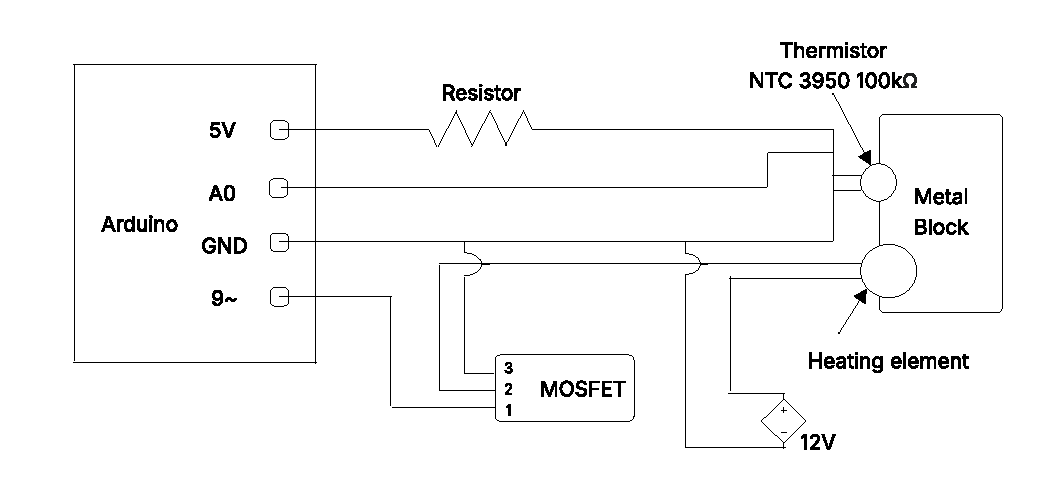
\includegraphics[width=0.8\textwidth]{PID_circuit_diagram}
    \caption{Wiring diagram of the experimental setup used for PID temperature control.}
    \label{fig:setup_diagram}
\end{figure}

\subsection{On-Off Control Baseline}
\label{subsec:on-off-control-baseline}

To establish a baseline response characteristic of the system, an on-off
control algorithm was implemented.
The heating element operated at maximum power until the thermistor registered
the set temperature of 65°C, at which point the heater was disabled until the
temperature dropped to the low temperature limit.
Temperature readings from the thermistor were recorded at approximately
one-second intervals and plotted as a function of time.
The expected behavior was characterized by a positive linear increase to a
peak above the set temperature, followed by a steeper decline back to the
lower temperature threshold, confirming proper circuit functionality.

\subsection{Proportional Control Implementation}
\label{subsec:proportional-control-implementation}

Following the baseline characterization, proportional control was implemented
using equation~\eqref{eq:power_proportional} to modulate heating power based
on the error between actual and set temperatures.
This approach reduced temperature oscillations by preventing full on-off
cycling and better maintained the temperature within the desired hysteresis band.
The proportionality constant \(k_p\) was initialized to 0.1 and incrementally
increased until measurable performance improvements were observed.
Despite these improvements, the system still exhibited a significant error
relative to the set temperature and continued to overshoot during each
oscillation cycle.

\subsection{System Response Time Characterization}
\label{subsec:system-response-time-characterization}

To optimize the integral control parameters, the system's reaction time was
determined using a step response method.
The reaction time was defined as the time required for the temperature to
reach 63\% of the total step change from baseline to target
temperature~\cite{step_response_wiki}.
A step input was applied by enabling the heating element to full power via the
MOSFET while continuously recording temperature measurements.
The initial temperature was measured using the thermistor, and the target
temperature was set to 5°C above this baseline value.
The time to reach the 63\% threshold was recorded as the system's response
time.
In accordance with laboratory guidelines~\cite{lab_guidelines}, the integral
action time constant was set to twice the measured response time to ensure
adequate system stabilization.

\subsection{Integral Control Refinement}
\label{subsec:integral-control-refinement}

Integral control was implemented to minimize the error and reduce the
oscillatory behavior observed with proportional control alone.
The integral constant \(k_i\) was initially set to approximately 0.0001 to
minimize the speed and magnitude of integral corrections, thereby reducing the
risk of integral windup~\cite{pid_integral_windup_controlcom} - a phenomenon
in which excessive error accumulation during actuator saturation leads to
overshooting and instability.
The integral constant was then gradually increased until the desired system
performance was achieved without overcorrection or instability.

\subsection{Derivative Control Optimization}
\label{subsec:derivative-control-optimization}

Derivative control was implemented to improve transient response and combat
sudden environmental temperature changes.
However, derivative action amplifies high-frequency noise in thermistor
measurements and measurement errors, potentially inducing unwanted
oscillations.
Therefore, the derivative constant \(k_d\) was initialized to 0.01 and
systematically decreased until the system ceased overreacting to measurement
noise while maintaining its ability to handle step changes in environmental
conditions.
Although derivative control is particularly beneficial for systems with
rapidly changing dynamics, its implementation in this relatively stable
thermal system required careful tuning to avoid amplifying measurement artifacts.

\subsection{Thermal Characterization}
\label{subsec:thermal-characterization}

Temperature-time response graphs were acquired at two different set
temperatures.
The voltage required to maintain each temperature was determined from the duty
cycle of the MOSFET at the stabilized portion of each response curve using
equation~\ref{eq:power_mosfet} to calculate the heat loss from the block.
Subsequently, the heating element was operated at full power using
Listing~\ref{lst:specific_heat_measurement} until a predetermined maximum
temperature was reached.
The time and power required to raise the temperature by 1°C were extracted
from these measurements.
These values were then substituted into equation~\ref{eq:specific_heat} to
determine the specific heat capacity of the test block.
Measurements at the two different temperatures allowed assessment of
temperature-dependent variations in specific heat capacity and estimation of
measurement uncertainty.